\documentclass[../cellseek_paper.tex]{subfiles}

\begin{document}

\section{Methods}

\subsection{System Architecture}

\begin{figure}[H]
  \centering
  \begin{tikzpicture}[
		% Define styles
		block/.style={rectangle, draw, thick, fill=blue!10, minimum width=3cm, minimum height=1.2cm, align=center},
		data/.style={rectangle, draw, thick, fill=green!10, rounded corners, minimum height=1.2cm, align=center},
		arrow/.style={->, >=stealth, thick},
		label/.style={text width=3cm, align=center}
	]

	% Input
	\node[data, fill=red!15] (input) at (0,0) {\textbf{Input}\\Microscopy Video\\$V = \{I_1, I_2, ..., I_T\}$};

	% Cellpose-SAM Block
	\node[block, right=2.5cm of input] (cellpose) {SAM Segmentation Module};
	\draw[arrow] (input) -- node[above, align=center] {\scriptsize Frame $I_t$} (cellpose);

	% Output of Cellpose-SAM
	\node[data, right=2.5cm of cellpose] (masks) {\textbf{Initial Masks}\\$M^{init}_t$ for frame $t$};
	\draw[arrow] (cellpose) -- (masks);

	% Adapted Cutie Block
	\node[block, below=2cm of cellpose] (cutie) {Cutie Temporal Tracker};

	% Memory flow (feedback loop)
	\node[data, left=1.2cm of cutie] (memory) {\textbf{Memory}\\$\mathcal{M}_{t-1}, \mathbf{Q}_{t-1}$};
	\draw[arrow] (memory) -- (cutie);

	% Flow from Masks to Cutie
	\draw[arrow] (masks.south) -- ++(0,-1) -| node[pos=0.25, above] {\scriptsize $M^{init}_t$} (cutie.north);

	% Final Output
	\node[data, fill=blue!15, right=2.5cm of cutie] (output) {\textbf{Output}\\Tracked Masks\\$M_t$ with IDs};
	\draw[arrow] (cutie) -- node[above] {\scriptsize $M_t, \mathbf{Q}_t$} (output);

	% Annotations
	\node[above=0.2cm of cellpose, label] {Automatic Segmentation};
	\node[below=0.2cm of cutie, label]{Temporal Tracking};

\end{tikzpicture}

  \caption{The CellSeek system architecture. The pipeline processes microscopy videos through two main stages: (1) the Cellpose-SAM module performs automatic instance segmentation on each frame, and (2) the adapted Cutie tracker maintains cell identities across time using only last-frame memory ($\mathcal{M}_{t-1}$) and object queries ($\mathbf{Q}_{t-1}$), which are updated each frame. This design eliminates complex parameter tuning while maintaining robust tracking performance.}
  \label{fig:architecture}
\end{figure}

CellSeek consists of three main components operating in a sequential pipeline: (1) Cellpose-SAM for initial cellular segmentation, and (2) adapted Cutie-based temporal tracking that uses only last-frame memory for efficient cell tracking. The system architecture is designed to minimize error propagation between components while maximizing the utilization of each module's specialized capabilities and the specific characteristics of cellular imaging.

The pipeline takes a microscopy video $V = \{I_1, I_2, \ldots, I_T\}$ where $I_t \in \mathbb{R}^{H \times W \times 3}$ represents the $t$-th frame, and outputs a sequence of segmentation masks $M = \{M_1, M_2, \ldots, M_T\}$ where $M_t \in \mathbb{Z}^{H \times W}$ contains integer cell identifiers for tracked cells at frame $t$.

\subsection{Cellpose-SAM: Cellular Segmentation Module}

\subsubsection{Architecture Overview}

Cellpose-SAM represents a strategic surgical transplant of the Segment Anything Model (SAM) \cite{kirillov2023segment} for biological instance segmentation. Rather than adapting SAM's prompt-based architecture, Cellpose-SAM takes a fundamentally different approach: it discards SAM's entire decoder and retains only the powerful pretrained image encoder, replacing the complex prompt-based decoder with a simple Cellpose-style \cite{stringer2021cellpose} output head.

\begin{figure}[H]
  \centering
  \begin{tikzpicture}[
    % Define styles
    encoder/.style={rectangle, draw, thick, fill=blue!20, minimum width=2.5cm, minimum height=1cm, align=center},
    decoder/.style={rectangle, draw, thick, fill=green!20, minimum width=2.5cm, minimum height=1cm, align=center},
    data/.style={rectangle, draw, thick, fill=gray!10, rounded corners, minimum height=0.8cm, align=center},
    arrow/.style={->, >=stealth, thick},
    dimension/.style={font=\scriptsize, above}
  ]

  % Input
  \node[data] (input) at (0,0) {Input Image\\$256 \times 256 \times 3$};

  % SAM Encoder
  \node[encoder, right=2cm of input] (vit) {Modified ViT-L\\Encoder\\24 Blocks};
  \draw[arrow] (input) -- node[above] {\scriptsize Patch 8×8} (vit);

  % Features
  \node[data, right=2cm of vit] (features) {Features\\$32 \times 32 \times 1024$};
  \draw[arrow] (vit) -- (features);

  % Cellpose Decoder
  \node[decoder, below=1.5cm of features] (decoder) {Cellpose\\Output Head};
  \draw[arrow] (features) -- node[right] {\scriptsize Transposed Conv} (decoder);

  % Flow outputs
  \node[data, left=1.5cm of decoder] (cellprob) {Cell Prob\\$256 \times 256$};
  \node[data, below=0.8cm of decoder] (dx) {Flow X\\$256 \times 256$};
  \node[data, right=1.5cm of decoder] (dy) {Flow Y\\$256 \times 256$};

  \draw[arrow] (decoder) -- (cellprob);
  \draw[arrow] (decoder) -- (dx);
  \draw[arrow] (decoder) -- (dy);

  % Mask reconstruction
  \node[decoder, below=1.5cm of dx, fill=orange!20] (recon) {Gradient\\Tracking};
  \draw[arrow] (cellprob) -- (recon);
  \draw[arrow] (dx) -- (recon);
  \draw[arrow] (dy) -- (recon);

  % Final output
  \node[data, below=1cm of recon, fill=yellow!20] (masks) {Instance\\Masks};
  \draw[arrow] (recon) -- (masks);

  % Annotations
  \node[above=0.3cm of vit, font=\small\bfseries] {SAM Foundation Model};
  \node[left=0.3cm of decoder, font=\small\bfseries, rotate=90] {Cellpose Framework};

\end{tikzpicture}

  \caption{Cellpose-SAM architecture overview. The model combines SAM's pretrained ViT-L encoder (adapted from 1024×1024 to 256×256 resolution) with Cellpose's flow field output head. Unlike SAM's complex prompt-based decoder, this hybrid approach uses simple transposed convolutions to generate cell probability maps and flow fields, which are then processed through Cellpose's gradient tracking algorithm to produce instance masks.}
  \label{fig:cellpose_sam_arch}
\end{figure}

This architectural choice leverages the broad visual knowledge from SAM's billion-mask pre-training while maintaining the efficiency and proven performance of the Cellpose framework for dense instance segmentation.

The architecture consists of three main components:

\begin{enumerate}
  \item \textbf{Modified ViT-L Encoder}: A customized version of SAM's Vision Transformer Large backbone, adapted for 256×256 microscopy images with architectural modifications for cellular imaging
  \item \textbf{Cellpose Output Head}: A simple transposed convolution layer that maps transformer features to Cellpose-specific flow field and probability representations
  \item \textbf{Cellpose Mask Reconstruction}: Algorithmic post-processing that converts flow fields into instance masks using gradient tracking dynamics
\end{enumerate}

\subsubsection{Modified ViT-L Encoder Architecture}

The Cellpose-SAM encoder is based on SAM's ViT-L backbone but includes several critical modifications optimized for microscopy imaging:

\textbf{Architectural Specifications:}
\begin{itemize}
  \item \textbf{Base Model}: ViT-L with 24 transformer blocks and 1024 embedding dimensions
  \item \textbf{Input Resolution}: Reduced from SAM's default 1024×1024 to 256×256, optimized for typical cellular imaging scales
  \item \textbf{Patch Size}: Reduced from 16×16 to 8×8 to preserve higher spatial resolution in feature representations
  \item \textbf{Attention Mechanism}: All layers use standard global self-attention (unlike SAM's hybrid local/global pattern), simplifying the architecture with minimal runtime penalty due to smaller input size
\end{itemize}

\textbf{Adaptation Process:}
\begin{itemize}
  \item \textbf{Patch Embedding}: Convolutional filters adapted via appropriate subsampling to work with 8×8 patches
  \item \textbf{Position Embeddings}: SAM's pretrained position embeddings downsampled by factor of 2 to match new grid dimensions (32×32 feature grid from 256÷8)
\end{itemize}

\subsubsection{Cellpose Output Head and Mask Reconstruction}

The decoder architecture abandons SAM's complex prompt-based design in favor of Cellpose's proven flow field approach:

\begin{algorithm}[H]
  \caption{Cellpose-SAM Processing Pipeline}
  \begin{algorithmic}[1]
    \REQUIRE Input image $I \in \mathbb{R}^{256 \times 256 \times 3}$
    \ENSURE Instance segmentation masks $\{M_1, M_2, \ldots, M_N\}$
    \STATE $\text{features} \leftarrow \text{Modified\_ViT\_L}(I)$ \COMMENT{Output: $[B, 1024, 32, 32]$}
    \STATE $\text{upsampled} \leftarrow \text{TransposedConv}(\text{features})$ \COMMENT{Upsample to $256 \times 256$}
    \STATE $[\text{cellprob}, \text{dx}, \text{dy}] \leftarrow \text{OutputHead}(\text{upsampled})$ \COMMENT{3-channel output}
    \STATE $\text{masks} \leftarrow \text{CellposeReconstruction}(\text{dx}, \text{dy}, \text{cellprob})$ \COMMENT{Gradient tracking}
    \RETURN $\text{masks}$
  \end{algorithmic}
\end{algorithm}

\textbf{Output Representations:}
\begin{itemize}
  \item \textbf{Cell Probability Map}: Single channel indicating probability of each pixel being at a cell center
  \item \textbf{Horizontal Flow (dx)}: X-component of vector pointing from each pixel to its cell center
  \item \textbf{Vertical Flow (dy)}: Y-component of vector pointing from each pixel to its cell center
\end{itemize}

\begin{figure}[H]
  \centering
  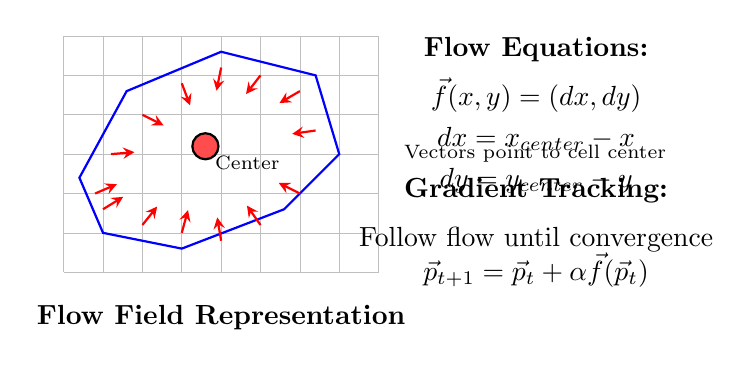
\begin{tikzpicture}[
    cell/.style={circle, draw, thick, fill=blue!30, minimum size=0.8cm},
    grid/.style={help lines, step=0.5cm, gray!50},
    arrow/.style={->, >=stealth, thick, red},
    center/.style={circle, draw, thick, fill=red!70, minimum size=0.3cm}
  ]

  % Grid
  \draw[grid] (0,0) grid (4,3);

  % Cell boundaries (rough outline)
  \draw[thick, blue] (0.5,0.5) -- (1.5,0.3) -- (2.8,0.8) -- (3.5,1.5) -- (3.2,2.5) -- (2.0,2.8) -- (0.8,2.3) -- (0.2,1.2) -- cycle;

  % Cell center
  \node[center] (center) at (1.8,1.6) {};

  % Flow vectors pointing to center
  \foreach \x/\y in {0.5/0.8, 1.0/0.6, 1.5/0.5, 2.0/0.4, 2.5/0.6, 3.0/1.0, 3.2/1.8, 3.0/2.3, 2.5/2.5, 2.0/2.6, 1.5/2.4, 1.0/2.0, 0.6/1.5, 0.4/1.0} {
      \pgfmathsetmacro{\dx}{1.8-\x}
      \pgfmathsetmacro{\dy}{1.6-\y}
      \pgfmathsetmacro{\len}{sqrt(\dx*\dx+\dy*\dy)}
      \pgfmathsetmacro{\ndx}{\dx/\len*0.3}
      \pgfmathsetmacro{\ndy}{\dy/\len*0.3}
      \draw[arrow] (\x,\y) -- +(\ndx,\ndy);
    }

  % Labels
  \node[below] at (2,-0.3) {\textbf{Flow Field Representation}};
  \node[right] at (4.2,1.5) {\scriptsize Vectors point to cell center};
  \node[below right] at (center) {\scriptsize Center};

  % Equations
  \node[align=center] at (6,2) {
    \textbf{Flow Equations:}\\[0.2cm]
    $\vec{f}(x,y) = (dx, dy)$\\[0.1cm]
    $dx = x_{center} - x$\\[0.1cm]
    $dy = y_{center} - y$
  };

  \node[align=center] at (6,0.5) {
    \textbf{Gradient Tracking:}\\[0.2cm]
    Follow flow until convergence\\
    $\vec{p}_{t+1} = \vec{p}_t + \alpha \vec{f}(\vec{p}_t)$
  };

\end{tikzpicture}

  \caption{Cellpose flow field visualization. The flow field vectors (arrows) point from each pixel toward the nearest cell center, creating a gradient field that guides the mask reconstruction process. Cell probability maps (shown as heat intensity) highlight regions likely to contain cell centers, while the gradient tracking algorithm follows flow vectors to group pixels into coherent instance masks.}
  \label{fig:flow_field}
\end{figure}

The final instance masks are generated through Cellpose's gradient tracking algorithm, where flow vectors are followed until convergence at cell centers, with pixels converging to the same center grouped into instance masks.

The model was extensively fine-tuned on aggregated biological datasets including Cellpose \cite{stringer2021cellpose}, TissueNet \cite{gjorevski2022tissue}, Omnipose \cite{cutler2022omnipose}, DeepBacs \cite{spahn2022deepbacs}, and MoNuSeg \cite{kumar2017dataset}. This specialized training process adapts SAM's general architecture to the specific morphological characteristics of cellular structures while preserving its inherent generalization capabilities across diverse imaging conditions.

\subsection{Temporal Tracking with Cutie}

\subsubsection{CellSeek Cutie Adaptation}

The temporal tracking component utilizes an adapted version of Cutie \cite{cheng2024putting}, a video object segmentation network that employs object-level memory reading to maintain consistent object identities across frames. For CellSeek, we have made a crucial adaptation to the original Cutie architecture by removing long-term memory and focusing exclusively on last-frame memory. This modification is specifically motivated by the characteristics of cellular imaging: cells within the same population exhibit highly similar morphological features, making long-term appearance memory redundant and potentially counterproductive.

Our adapted Cutie architecture addresses the unique challenges of cell tracking by leveraging the fact that cellular identity is better maintained through spatial proximity and immediate temporal context rather than accumulated appearance history. The simplified architecture consists of three core components:

\begin{enumerate}
  \item \textbf{Query-based Object Transformer}: Adapts object queries for high-level object representation
  \item \textbf{Last-Frame Memory Reader}: Retrieves relevant information exclusively from the previous frame
  \item \textbf{Foreground-Background Masked Attention}: Cleanly separates object semantics from background
\end{enumerate}

\subsubsection{Memory Architecture for Cell Tracking}

Unlike the original Cutie which maintains extensive temporal memory banks, our adaptation employs a streamlined memory system that stores only the most recent frame information. This design choice provides several advantages specific to cell tracking:

\begin{itemize}
  \item \textbf{Reduced Memory Footprint}: Elimination of long-term memory significantly reduces computational requirements
  \item \textbf{Improved Specificity}: Cells of the same type share nearly identical appearances, making long-term memory potentially confusing rather than helpful
  \item \textbf{Enhanced Real-time Performance}: Simplified memory management enables faster processing suitable for interactive applications
  \item \textbf{Reduced Error Accumulation}: Shorter memory prevents the propagation of segmentation errors over long temporal sequences
\end{itemize}

\begin{figure}[H]
  \centering
  \begin{tikzpicture}[
    memory/.style={rectangle, draw, thick, fill=blue!20, minimum width=2cm, minimum height=0.8cm, align=center},
    memory_light/.style={rectangle, draw, thick, fill=blue!10, minimum width=2cm, minimum height=0.8cm, align=center},
    processor/.style={rectangle, draw, thick, fill=green!20, minimum width=2.5cm, minimum height=1cm, align=center},
    arrow/.style={->, >=stealth, thick, color=black!70},
    disabled_arrow/.style={->, >=stealth, thick, color=red!50, dashed},
    title/.style={font=\large\bfseries}
  ]

  % Original Cutie (top)
  \node[title] at (3,6) {Original Cutie Architecture};

  % Long-term memory stack
  \node[memory] (mem1) at (0,5) {Frame $t-5$};
  \node[memory] (mem2) at (0,4.2) {Frame $t-4$};
  \node[memory] (mem3) at (0,3.4) {Frame $t-3$};
  \node[memory] (mem4) at (0,2.6) {Frame $t-2$};
  \node[memory] (mem5) at (0,1.8) {Frame $t-1$};

  % Memory reader
  \node[processor] (reader1) at (3,3.5) {Memory\\Reader};

  % Improved arrows from all memories - connecting to specific anchor points
  \draw[arrow] (mem1.east) -- (reader1.west);
  \draw[arrow] (mem2.east) -- (reader1.west);
  \draw[arrow] (mem3.east) -- (reader1.west);
  \draw[arrow] (mem4.east) -- (reader1.west);
  \draw[arrow] (mem5.east) -- (reader1.west);

  % Current frame
  \node[memory, fill=yellow!30] (current1) at (6,3.5) {Current\\Frame $t$};
  \draw[arrow] (reader1.east) -- (current1.west);

  % Separator line
  \draw[thick, dashed] (-1,0.5) -- (7,0.5);

  % CellSeek Adapted Cutie (bottom)
  \node[title] at (3,-0.5) {CellSeek Adapted Cutie};

  % Only last frame memory
  \node[memory_light, pattern=north east lines] (old_mem1) at (0,-1.5) {Frame $t-5$};
  \node[memory_light, pattern=north east lines] (old_mem2) at (0,-2.3) {Frame $t-4$};
  \node[memory_light, pattern=north east lines] (old_mem3) at (0,-3.1) {Frame $t-3$};
  \node[memory_light, pattern=north east lines] (old_mem4) at (0,-3.9) {Frame $t-2$};
  \node[memory, fill=orange!30] (last_mem) at (0,-4.7) {Frame $t-1$};

  % Simplified memory reader
  \node[processor, fill=orange!20] (reader2) at (3,-3) {Last-Frame\\Memory Reader};

  % Active arrow from only last frame
  \draw[arrow] (last_mem.east) -- (reader2.west);

  % Disabled arrows from old memories (optional - shows what's not used)
  \draw[disabled_arrow] (old_mem1.east) -- (reader2.west);
  \draw[disabled_arrow] (old_mem2.east) -- (reader2.west);
  \draw[disabled_arrow] (old_mem3.east) -- (reader2.west);
  \draw[disabled_arrow] (old_mem4.east) -- (reader2.west);

  % Current frame
  \node[memory, fill=yellow!30] (current2) at (6,-3) {Current\\Frame $t$};
  \draw[arrow] (reader2.east) -- (current2.west);

  % Cross out old memories
  \foreach \i in {1,2,3,4} {
      \draw[thick, red, opacity=0.7] (old_mem\i.south west) -- (old_mem\i.north east);
      \draw[thick, red, opacity=0.7] (old_mem\i.south east) -- (old_mem\i.north west);
    }

  % Benefits annotation
  \node[align=left, font=\small] at (10,0.5) {
    \textbf{Benefits:}\\
    • Reduced memory\\
    • Faster processing\\
    • Less error accumulation\\
    • Cell-specific optimization
  };

\end{tikzpicture}

  \caption{Memory architecture comparison between original Cutie and CellSeek adaptation. Original Cutie maintains extensive long-term memory banks that accumulate features over many frames, while CellSeek's adaptation uses only last-frame memory to avoid confusion from morphologically similar cells and reduce computational overhead.}
  \label{fig:memory_comparison}
\end{figure}

\subsubsection{Last-Frame Memory Representation}

Our adapted Cutie maintains a simplified memory structure that focuses on immediate temporal context:

\begin{align}
  \mathcal{M}_{current} & = \{\mathbf{k}^{t-1}, \mathbf{v}^{t-1}\}_{t-1} \\
  \mathcal{Q}_{objects} & = \{\mathbf{q}_i^{obj}\}_{i=1}^{N_{cells}}
\end{align}

where $\mathbf{k}^{t-1}, \mathbf{v}^{t-1}$ represent key-value features from frame $t-1$ only, and $\mathbf{q}_i^{obj}$ represents object queries for each tracked cell that are updated frame-by-frame without long-term accumulation.

\begin{figure}[H]
  \centering
  \begin{tikzpicture}[
    frame/.style={rectangle, draw, thick, fill=blue!20, minimum width=1.5cm, minimum height=2cm, align=center},
    memory/.style={rectangle, draw, thick, fill=orange!30, minimum width=1.2cm, minimum height=0.6cm, align=center},
    query/.style={ellipse, draw, thick, fill=green!30, minimum width=1cm, minimum height=0.5cm, align=center},
    arrow/.style={->, >=stealth, thick},
    time_arrow/.style={->, >=stealth, very thick, blue}
  ]

  % Timeline
  \draw[time_arrow] (0,0) -- (12,0);
  \node[below] at (6,-0.5) {\textbf{Time}};

  % Frames
  \node[frame] (f1) at (2,2) {Frame\\$t-2$};
  \node[frame] (f2) at (5,2) {Frame\\$t-1$};
  \node[frame] (f3) at (8,2) {Frame\\$t$};
  \node[frame] (f4) at (11,2) {Frame\\$t+1$};

  % Memory blocks (only from previous frame)
  \node[memory] (m1) at (5,4) {$\mathcal{M}_{t-1}$};
  \node[memory] (m2) at (8,4) {$\mathcal{M}_{t}$};
  \node[memory] (m3) at (11,4) {$\mathcal{M}_{t+1}$};

  % Object queries
  \node[query] (q1) at (5,0.5) {$\mathbf{Q}_{t-1}$};
  \node[query] (q2) at (8,0.5) {$\mathbf{Q}_{t}$};
  \node[query] (q3) at (11,0.5) {$\mathbf{Q}_{t+1}$};

  % Memory flow (only last frame)
  \draw[arrow, red, thick] (m1) -- (f3);
  \draw[arrow, red, thick] (m2) -- (f4);

  % Query updates
  \draw[arrow, green!70!black] (q1) -- (q2);
  \draw[arrow, green!70!black] (q2) -- (q3);

  % Memory updates
  \draw[arrow, orange!70!black] (f2) -- (m1);
  \draw[arrow, orange!70!black] (f3) -- (m2);
  \draw[arrow, orange!70!black] (f4) -- (m3);

  % Cross out older memories to show they're not used
  \node[memory, pattern=north east lines, opacity=0.3] (old_m) at (2,4) {$\mathcal{M}_{t-2}$};
  \draw[thick, red, opacity=0.7] (old_m.south west) -- (old_m.north east);
  \draw[thick, red, opacity=0.7] (old_m.south east) -- (old_m.north west);

  % Legend
  \node[align=left, font=\scriptsize] at (-1.5,3) {
    \textcolor{red}{$\longrightarrow$} Memory Read\\
    \textcolor{green!70!black}{$\longrightarrow$} Query Update\\
    \textcolor{orange!70!black}{$\longrightarrow$} Memory Store
  };

\end{tikzpicture}

  \caption{Temporal tracking timeline showing last-frame-only memory architecture. Unlike traditional approaches that accumulate memory over many frames, CellSeek's adapted Cutie maintains only the immediate previous frame memory ($\mathcal{M}_{t-1}$) for processing frame $t$. Object queries ($\mathbf{Q}_t$) are updated continuously while older memory states are discarded to prevent confusion from morphologically similar cells.}
  \label{fig:temporal_timeline}
\end{figure}

\subsubsection{Tracking Algorithm}

The adapted Cutie tracking process operates with last-frame memory only:

\begin{algorithm}[H]
  \caption{CellSeek Adapted Cutie Tracking}
  \begin{algorithmic}[1]
    \REQUIRE Current frame $I_t$, previous frame features $\mathcal{M}_{t-1}$, object queries $\mathbf{Q}_{t-1}$
    \ENSURE Predicted mask $M_t$, updated queries $\mathbf{Q}_t$
    \STATE $\mathbf{f}_t \leftarrow \text{FeatureExtractor}(I_t)$
    \STATE $\mathbf{Q}_t^{init} \leftarrow \text{QueryUpdate}(\mathbf{Q}_{t-1}, \mathcal{M}_{t-1})$
    \STATE $\mathbf{f}_t^{enhanced} \leftarrow \text{QueryTransformer}(\mathbf{Q}_t^{init}, \mathbf{f}_t)$
    \STATE $M_t \leftarrow \text{MaskDecoder}(\mathbf{f}_t^{enhanced})$
    \STATE $\mathcal{M}_t \leftarrow \text{ExtractFeatures}(I_t, M_t)$ \COMMENT{Store only current frame}
    \STATE $\mathbf{Q}_t \leftarrow \text{UpdateQueries}(\mathbf{Q}_t^{init}, M_t)$
    \RETURN $M_t, \mathbf{Q}_t$
  \end{algorithmic}
\end{algorithm}

\end{document}
